\section{Finding 4 - SSH Root Access via less}
\hrule
\begin{table}[htb]
    \renewcommand{\arraystretch}{1.5}
    \begin{tabular*}{\textwidth}{|>{\columncolor{red!15}}p{3cm}|p{17.2cm}|}
    \textbf{Finding} & \textbf{SSH Root Access}\\
    Risk& High\\
    Category& Access Controls, Privilege Escalation\\
    Impact& An attacker is able to gain SSH root access.\\ 
    Description& After logging into the user account ''bluey'' the command ''sudo -l'' illustrates the users privileges. 
    \newline
    \newline
    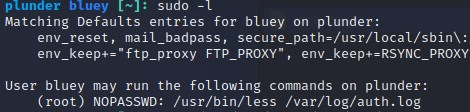
\includegraphics[width=0.73\textwidth]{sudo_l.jpg}
    \newline
    The command disclosed that ''bluey'' has root access for the command: ''/usr/bin/less /var/log/auth.log'' without as password. Although there was initially a misinterpretation of the output when attempting to run ''sudo less'' on a file or accessing the ''auth.log'' file, the command ultimately worked. Upon conducting research on methods for escalating privileges, it was discovered that it is possible to input ''! /bin/bash'' into the less command line, which will grant root access to the bash.
    \newline
    \newline
    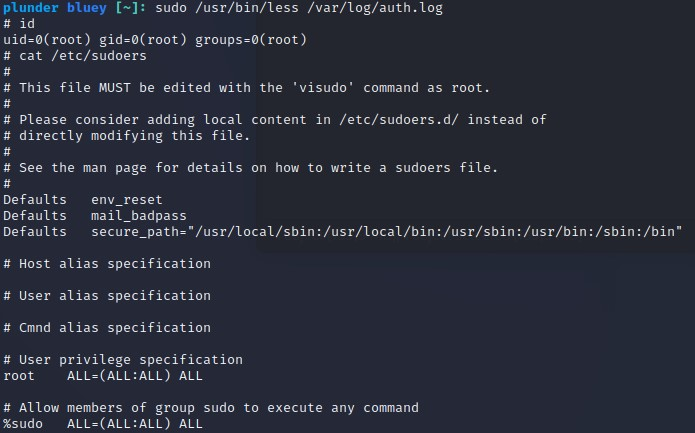
\includegraphics[width=0.73\textwidth]{root_access.jpg}
    \newline
    Executing the command ''id'' will display the current user. The graphic above illustrates that the current user has a uid of zero, which corresponds to the root user.
    The root user has all privileges as shown under the headline ''privilege specification''.
    \\
    \end{tabular*}
    \end{table}
    
